\documentclass[12pt, a4paper, oneside]{article}
\usepackage[T1]{fontenc}
\usepackage{amsmath, amsthm, amssymb, bm, booktabs, color, enumitem, float, graphicx, hyperref, mathrsfs, titling}
\usepackage[UTF8, scheme = plain]{ctex}
\usepackage{graphicx, minted, listings, subfigure}
\usepackage{grffile}
\title{\textbf{Homework 6}}
\setlength{\droptitle}{-10em}
\author{PENG Qiheng \\ Student ID\: 225040065}
\date{\today}
\linespread{1.5}
\newcounter{problemname}
\newenvironment{problem}{\stepcounter{problemname}\par\noindent{Problem \arabic{problemname}. }}{\par}
\newenvironment{solution}{\par\noindent{Solution. }}{\par}

\begin{document}

\maketitle

\begin{problem}
\begin{enumerate}[label = (\alph*)]
    \item  When $x > 0$, $f'(x) = \frac{3}{2} x^{\frac{1}{2}}$ \\
    And we can easily see $f'(0) = 0$
    \begin{gather}
        \notag ||\nabla f(x) - \nabla f(0)|| = \frac{3}{2} x^{\frac{1}{2}} \le L||x|| = Lx \\
        \notag \Rightarrow \frac{3}{2} \le L x^{\frac{1}{2}}
    \end{gather}
    When $x \to 0^+$, there is no such finite $L > 0$ satisfies the formulation. \\
    So $f$ is not Lipschitz smooth.
    \item  \begin{gather}
        \notag x_1 = x_0 - \bar \alpha f'(x_0)
        \notag \text{If } x_0 > 0 \text{, } f'(x_0) = \frac{3}{2} x_0^{\frac{1}{2}} \\
        \notag \Rightarrow x_1 = x_0 - \bar \alpha \frac{3}{2} x_0^{\frac{1}{2}} = x_0^{\frac{1}{2}} \left( x_0^{\frac{1}{2}} - \frac{3}{2} \bar \alpha \right) \\
        \notag f(x_1) = x_0^{\frac{3}{4}} \left | x_0^{\frac{1}{2}} - \frac{3}{2} \bar \alpha \right |^{\frac{3}{2}} \\
        \notag f(x_1) - f(x_0) = x_0^{\frac{2}{3}} \left ( x_0^{\frac{3}{4}} {\left | x_0^{\frac{1}{2}} - \frac{3}{2} \bar \alpha \right |}^{\frac{3}{2}} - 1 \right ) \ge 0 \\
        \notag \Rightarrow x_0 \le \frac{9}{16} \bar \alpha
    \end{gather}
    Similarly, when $x_0 < 0$, we need $x_0 \le \frac{9}{16} \bar \alpha$. \\
    If $x_0 = 0$, since $f'(0) = 0$, $\forall x_1, f(x_1) \ge f(x_0)$. \\
    Thus, for any constant step size $\bar \alpha > 0$, there exists an initial point $x_0$ such that $f(x_1) \ge f(x_0)$.
\end{enumerate}
\end{problem}

\newpage
\begin{problem}
\begin{enumerate}[label = (\alph*)]
    \item  \begin{enumerate}[label = (\roman*)]
        \item  \begin{gather}
            \notag \nabla f(x) = 2Ax = \begin{bmatrix}
                4x_1 \\
                10x_2
            \end{bmatrix} \\
            \notag x_1 = x_0 - \alpha_0 \nabla f(x_0) = \begin{bmatrix}
                0.6 \\
                0
            \end{bmatrix}
        \end{gather}
        \item  \begin{gather}
            \notag d_0 = - \nabla f(x_0) = \begin{bmatrix}
                -4 \\
                -10
            \end{bmatrix} \\
            \notag \alpha_0 = - \frac{d_0^T d_0}{2 d_0^T A d_0} = \frac{116}{1064} = \frac{29}{266} \\
            \notag x_1 = x_0 + \alpha_0 \nabla f(x_0) = \begin{bmatrix}
                \frac{75}{133} \\
                - \frac{12}{133}
            \end{bmatrix}
        \end{gather}
        \item  When $\alpha_0 = 1$,
        \begin{gather}
            \notag z_1 = f(x_0 - \alpha_0 \nabla f(x_0)) = 423 \\
            \notag z_2 = f(x_0) - \gamma \alpha_0 {||\nabla f(x_0)||}^2 = -51
        \end{gather}
        Since $z_1 > z_2$, the Armijo condition is not satisfied. \\
        When $\alpha_0 = \sigma = 0.2$,
        \begin{gather}
            \notag z_1 = f(x_0 - \alpha_0 \nabla f(x_0)) = 5.08 \\
            \notag z_2 = f(x_0) - \gamma \alpha_0 {||\nabla f(x_0)||}^2 = -4.6
        \end{gather}
        Since $z_1 > z_2$, the Armijo condition is not satisfied. \\
        When $\alpha_0 = \sigma^2 = 0.04$,
        \begin{gather}
            \notag z_1 = f(x_0 - \alpha_0 \nabla f(x_0)) = 3.2112 \\
            \notag z_2 = f(x_0) - \gamma \alpha_0 {||\nabla f(x_0)||}^2 = 4.68
        \end{gather}
        Since $z_1 < z_2$, the Armijo condition is satisfied. \\
        Thus, the step size determined by the Armijo rule is $\alpha_0 = 0.04$, and $x_1 = \begin{bmatrix} 0.84 \\ 0.6 \end{bmatrix}$.
\end{enumerate}
    \item  The code is in \texttt{p2.py}. The final outputs after running the code are as follows:
    \begin{figure}[H]
        \centering
        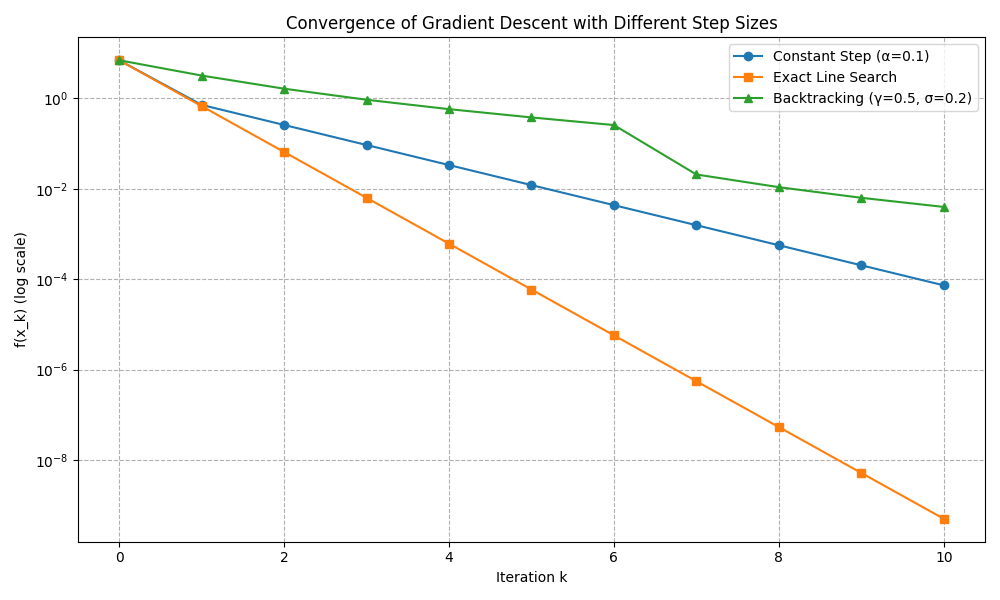
\includegraphics[width=0.8\textwidth]{../code/p2.png}
    \end{figure}
\end{enumerate}
\end{problem}

\newpage
\begin{problem}
\begin{enumerate}[label = (\alph*)]
    \item  \begin{gather}
        \notag \begin{cases}
            \frac{\partial f}{\partial x} = x^{\frac{1}{3}} + x + y = 0 \\
            \frac{\partial f}{\partial y} = x + y = 0
        \end{cases} \Rightarrow \begin{cases}
            x = 0 \\
            y = 0
        \end{cases} \\
        \notag H = \begin{bmatrix}
            \frac{1}{3} x^{-\frac{2}{3}} + 1 & 1 \\
            1 & 1
        \end{bmatrix}, \quad H(0, 0) = \begin{bmatrix}
            1 & 1 \\
            1 & 1
        \end{bmatrix}
    \end{gather}
    Since $H(0, 0)$ is positive semidefinite and $f$ is a convex function, $(0, 0)$ is a global minimum.
    \item  \begin{gather}
        \notag d = - \left ( \nabla^2 f(x, y) \right )^{-1} \nabla f(x, y) = - \begin{bmatrix}
            3x_k \\
            -2x_k + y_k
        \end{bmatrix} \\
        \notag x_{k+1} = x_k + d_1 = -2x_k \\
        \notag y_{k+1} = y_k + d_2 = 2x_k
    \end{gather}
    Thus, we can have $x_k \ne 0 \Rightarrow x_{k+1} \ne 0$, i.e., Newton's method will not converge if the initial point is not the optimal point.
    \item  $\Omega = {(x, y) : x + y = 1} = {z : az = b}$, \\
    while $z = {(x, y)}^{-1}, a = {(1, 1)}^{-1}, b = 1$. \\
    Take an unconstrainted step:
    \begin{gather}
        \notag z_{k+1}' = z_k - \alpha_k \nabla f(z_k) = - \begin{bmatrix}
            -\alpha_k x_k^{\frac{1}{3}} + (1 - \alpha_k)x_k - \alpha_k y_k \\
            - \alpha_k x_k + (1 - \alpha_k)y_k
        \end{bmatrix}
    \end{gather}
    \begin{align}
        \notag z_{k+1} & = P_{\Omega} (z_{k+1}') \\
        \notag & = z_{k+1}' - \frac{a^T z_{k+1}' - b}{{||a||}^2}a \\
        \notag & = \frac{1}{2} \begin{bmatrix}
            - \alpha_k x_k^{\frac{1}{3}} + x_k - y_k - 1 \\
            \alpha_k x_k^{\frac{1}{3}} - x_k + y_k - 1
        \end{bmatrix}
    \end{align}
    Thus, $\begin{bmatrix} x_{k+1} \\ y_{k+1} \end{bmatrix} = \begin{bmatrix} - \alpha_k x_k^{\frac{1}{3}} + x_k - y_k - 1 \\ \alpha_k x_k^{\frac{1}{3}} - x_k + y_k - 1 \end{bmatrix}$.
\end{enumerate}
\end{problem}

\newpage
\begin{problem}
\begin{enumerate}[label = (\alph*)]
    \item  Let $y = p + tv$, then
    \begin{gather}
        \notag \min_y f = \frac{1}{2} {||y - x||}^2 = \frac{1}{2} {||p + tv - x||}^2 \\
        \notag = \frac{\partial f}{\partial t} = v^T (p + tv - x) = 0 \\
        \notag \Rightarrow t^* = \frac{v^T (x - p)}{{||v||}^2} \\
        \notag \Rightarrow P_L(x) = y^* = p + \frac{v^T (x - p)}{{||v||}^2} v
    \end{gather}
    \item  \begin{gather}
        \notag P_L(x) = \text{argmin}_{y \in L} {||y - x||}^2
    \end{gather}
    If $y^* = P_L(x) \in B$,
    \begin{align}
        \notag y^* & = \text{argmin}_{y \in (L\cap B)} {||y - x||}^2 \\
        \notag & = \text{argmin}_{y \in C} {||y - x||}^2 \\
        \notag & = P_C(x)
    \end{align}
    Thus, when $P_L(x) \in B$, $P_C(x) = P_L(x)$.
\end{enumerate}
\end{problem}

\end{document}